\section{Results}
\label{sec:results}

Everything below uses the parameter set in Appendix~\ref{app:params}, and every
number can be reproduced from the simulator.

\subsection{Stage trajectories}

Figure~\ref{fig:stages} shows capability, regulation and observability for the
eight canonical stage configurations. Table~\ref{tab:stagecheck} sets what each
stage actually did against what that stage is \emph{defined} to do. This is a
low bar, and we report it because it is a bar models fail all the time without
anyone noticing --- a stage called ``collapse'' that quietly grows is the sort
of thing that survives for years inside a plausible-looking plot.

Two configurations reward a closer look. Stage~1, the early technological
phase, has no regulatory damping at all, so capability reduces to a plain
logistic equation and hits its analytic limits exactly: $\Icap \to aA/s_I = 3.0$
and $\Obs \to 1-e^{-\lambda \Icap} = 0.5934$ (Appendix~\ref{app:closed}).
Stage~4a drives regulation down to $\Reg_\infty = 0.0438$, below the collapse
threshold $\Rmin=0.05$ --- and it gets there \emph{without $\Reg$ ever going
negative}. Collapse happens by regulatory exhaustion, the mechanism we meant to
model, rather than by a sign flip in the damping term, which is the mechanism we
did not.

\begin{figure}[tb]
\centering
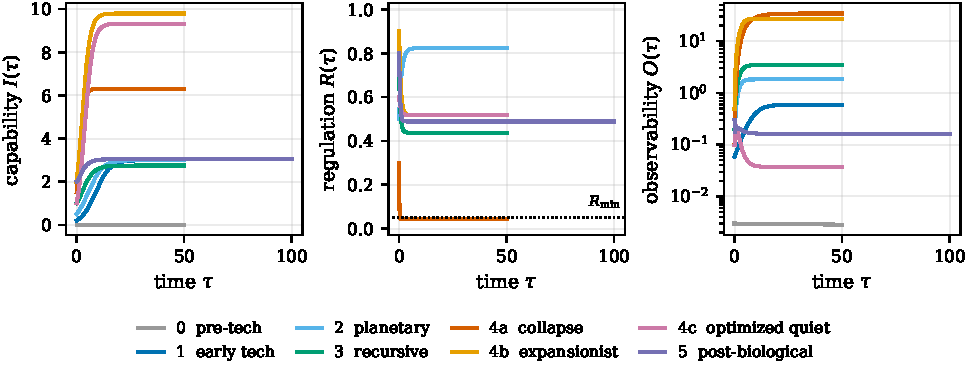
\includegraphics[width=\textwidth]{figures/fig05_stage_trajectories.pdf}
\caption{Capability, regulation and observability across the eight stage
configurations. Regulation stays inside $[0,1]$ by
Proposition~\ref{prop:reg}. Observability is plotted logarithmically and stays
strictly positive by Proposition~\ref{prop:obs}, spanning nearly five orders of
magnitude from the quietest stage to the loudest.}
\label{fig:stages}
\end{figure}

\begin{table}[tb]
\centering\small
\caption{What each stage was specified to do, against what it did.}
\label{tab:stagecheck}
\begin{tabular}{@{}llll@{}}
\toprule
Stage & Specified behaviour & Simulated & Regime \\
\midrule
0   & $\mathrm{d}\Icap/\mathrm{d}\tau\approx0$, no signature & $\Icap=0.010$, $\Obs=0.003$ & pre-detectable \\
1   & $\Icap\to aA/s_I$, $\Obs$ rising & $\Icap=3.0000$, $\Obs=0.5934$ & visible technological \\
2   & capability grows, $\Obs$ still rising & $\Icap=3.000$, $\Obs:0.10\to1.82$ & visible technological \\
3   & full model, recursion active & $\Icap=2.75$, $\Obs=3.43$ & visible technological \\
4a  & regulation collapses & $\Reg\to0.0438<\Rmin$, $\Reg\geq0$ & collapse proxy \\
4b  & high $\Icap$, high $\Obs$ sustained & $\Icap=9.80$, $\Obs=27.0$ & expansionist visible \\
4c  & $\Obs$ peaks, then declines & $0.100\to0.231\to0.037$ & optimized low-observable \\
5   & speculative & $\Icap=3.04$, $\Obs:0.30\to0.16$ & visible technological \\
\bottomrule
\end{tabular}
\end{table}

\subsection{Peak-then-decline is derived, not imposed}
\label{sec:derived}

This is the central result, and Figure~\ref{fig:suppression} is the whole
argument in one picture. Both panels are the \emph{same} stage-4c
configuration. Only the form of the suppression term differs.

Panel (a) uses an absolute suppression term, $-mC-nS$, whose rate does not
depend on $\Obs$ at all. Observability passes through zero at $\tau\approx0.3$
and then just keeps going, reaching $-1431$ by the end of the run. And here is
the part that should bother you: under the criteria of Table~\ref{tab:regimes}
that trajectory is still labelled ``optimized low-observable'', because the
classifier looks at $\Obs < \Odet$ and finds it satisfied. The label is
arithmetically correct and physically empty. The civilization is not quiet. It
has fallen off the bottom of the model.

Panel (b) uses the fractional form of Eq.~\eqref{eq:dO}. Observability rises
from $0.100$ to a peak of $0.231$ at $\tau=0.65$, then decays to $0.037$: below
the detection threshold, above the thermodynamic floor, and strictly positive
the entire time.

Now, why does it decline? Nothing in this configuration picks a peaked
functional form --- $\Obs$ is integrated, not evaluated from some curve we chose
in advance. The decline comes straight out of Eq.~\eqref{eq:decline}.
Compression and stealth scale as $\Icap^{2}\Reg$ while production scales as
$\Icap$, so the quasi-steady observability $\Obs^{*} \sim 1/(\Icap\Reg)$ has to
fall as capability grows. The civilization gets harder to see because its
efficiency outruns its output. That is a mechanism, not a stipulation.
\Plausible

The distinction is the whole answer to the standing objection against
low-observability accounts of the Great Silence --- that they assume the very
thing they set out to explain. A model that selects a peaked $\Obs(\Icap)$ does
assume it, and the objection lands. A model that gets the peak out of the ratio
of two independently motivated terms does not, and has to be attacked somewhere
else: on whether the required scaling separation is physically plausible. We
think that is a much better argument to be having.

\begin{figure}[tb]
\centering
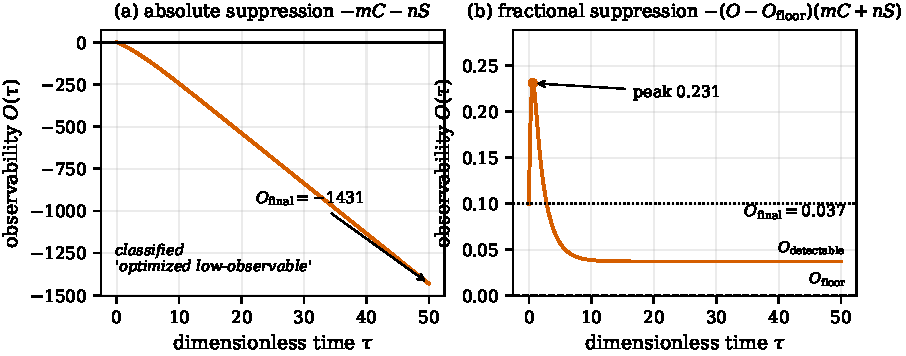
\includegraphics[width=\textwidth]{figures/fig07_suppression_comparison.pdf}
\caption{Why the form of the suppression term decides everything. Both panels
are the same configuration. (a) With absolute suppression the trajectory passes
through zero and dives, spending the entire run inside the shaded region the
model's own thermodynamics forbid --- and it is \emph{still} classified
``optimized low-observable''. (b) With fractional suppression and a
thermodynamic floor, the same configuration gives a genuine peak-then-decline,
bounded below. The decline is derived from suppression outscaling production,
not imposed by choosing a peaked profile.}
\label{fig:suppression}
\end{figure}

\subsection{Robustness across observability models}

Figure~\ref{fig:obsmodels} shows the four static observability models from
Table~\ref{tab:registry}: one rising, one falling, one peaked, one switching on
at a threshold. The framework admits all four.

The useful robustness question is not which curve is right. Nobody knows which
curve is right. The question is whether a conclusion survives changing it. The
low-observability regime is reachable under the peaked and decreasing models and
under the dynamical form of Eq.~\eqref{eq:dO}. It is \emph{not} reachable under
the increasing model, which instead gives the expansionist-visible regime we see
in stage~4b.

We count that as the framework working correctly. A model in which every
functional choice led to the same conclusion would not be testing anything at
all; it would be a machine for producing the answer we already had.
\Established

\begin{figure}[tb]
\centering
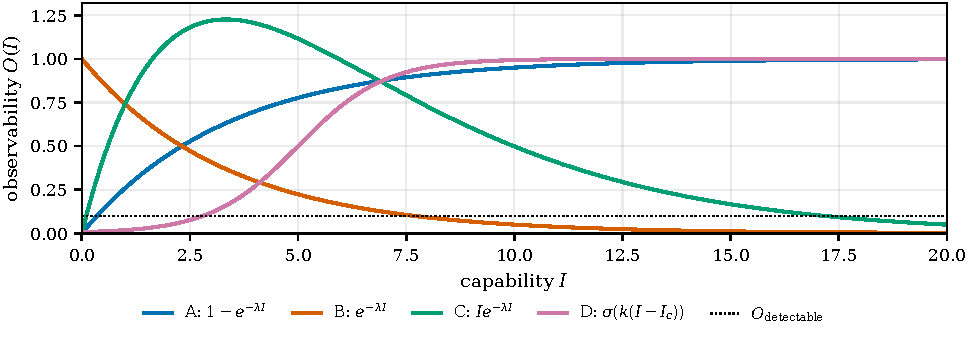
\includegraphics[width=\textwidth]{figures/fig06_observability_models.pdf}
\caption{The four interchangeable static observability models: A rises and
saturates, B falls from the start, C rises then falls, D switches on at a
threshold. Any conclusion about the Great Silence has to be reported together
with the model that produced it --- the low-observability regime does not arise
under model~A at all.}
\label{fig:obsmodels}
\end{figure}

\subsection{Phase structure}

Figure~\ref{fig:phase} puts the trajectories in the $(\Icap,\Reg)$ plane.
Because regulation is confined to $[0,1]$, the reachable phase space is a
bounded strip rather than a half-plane, and that makes the regime boundaries
directly readable off the picture: the vertical line at $\Iadv$ separates
pre-advanced from advanced capability, and the horizontal line at $\Rmin$ marks
regulatory exhaustion.

The branch structure of Figure~\ref{fig:ladder} is visible here as geometry.
Configurations that start in the same place separate according to whether
regulation holds: those keeping $\Reg\gtrsim0.5$ run to the right along the
strip into the advanced regimes, while stage~4a drops to the lower boundary and
trips the collapse proxy. \Hypothetical

\begin{figure}[tb]
\centering
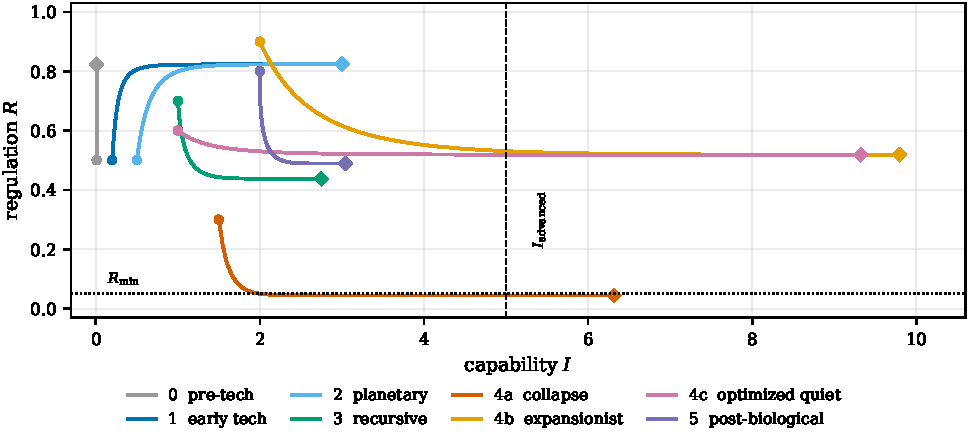
\includegraphics[width=\textwidth]{figures/fig08_phase_portrait.pdf}
\caption{Phase portrait in the capability--regulation plane. Circles mark
initial conditions, diamonds mark final states. Regulation is bounded to
$[0,1]$, so the reachable region is a strip, and the collapse boundary $\Rmin$
is approached but never crossed into negative values.}
\label{fig:phase}
\end{figure}

\subsection{Decomposing the silence}

Finally, Eq.~\eqref{eq:decomp} lets us ask which factor a null result actually
constrains. Take stage~4c, with $\Obs=0.037$, $\kappa=1$ and $\Psearch=0.5$. The
detection probability for a single civilization is
\begin{equation}
  \Pdet = \big(1-e^{-\kappa \Obs}\big)\Psearch = 0.018 ,
\end{equation}
against $\Pdet = 0.50$ for the expansionist stage~4b at $\Obs=27$. So the same
underlying population is about 27 times less likely to be detected in the quiet
regime than in the loud one --- with no change in $\Ntrue$ whatsoever, and
nobody going extinct. \Hypothetical

We want to be careful about what this does not show. It does not show that
civilizations are quiet, and it certainly does not show that quietness explains
the Great Silence. What it shows is narrower and, we think, more useful: under
this framework a null result is compatible with a wide range of $\Ntrue$, so
anyone attributing non-detection to rarity is making an argument about $\Obs$
and $\Psearch$ whether they say so or not. Usually they do not say so.
